\documentclass[a4paper,twoside]{article}

\usepackage{epsfig}
\usepackage{subfigure}
\usepackage{calc}
\usepackage{amssymb}
\usepackage{amstext}
\usepackage{amsmath}
\usepackage{amsthm}
\usepackage{multicol}
\usepackage{pslatex}
\usepackage{apalike}
%\usepackage[draft]{hyperref} %%
\usepackage{hyperref} %%
\usepackage{url} %%
\usepackage[hang,flushmargin]{footmisc}
\usepackage{SCITEPRESS}     % Please add other packages that you may need BEFORE the SCITEPRESS.sty package.



\subfigtopskip=0pt
\subfigcapskip=0pt
\subfigbottomskip=0pt

\begin{document}

%\title{GDPR  \subtitle{In Letter \& Spirit} }
%\title{Right to be Forgotten \textit{w.r.t.} Social Networks}
\title{Efficacy of \textit{Right to be Forgotten} in Social Networks}
\author{} % blind review

% \author{\authorname{Vishwas T. Patil, RK Shyamasundar}
% \affiliation{ISRDC, CSE, IIT Bombay, Mumbai 400076, India.}
% \email{\{ivishwas, shyamasundar\}@gmail.com}
% }

\keywords{identity, linkability, privacy, social networks, data
  governance, GDPR}

\abstract{
  Online social networks like Facebook have become silent witness to
  our online activities either by our consent or by our desire to
  avail services for free. Being witness to our activities they
  construct so much knowledge about us that they can predict our
  intentions, priorities, personal traits. Realizing the potential
  privacy implications of such an aggregation of user data, European
  Union devised GDPR. One of the core tenets of this regulation is
  \textit{right to be forgotten} and we argue that it will have little
  or no impact when invoked on Facebook platform. We investigate the
  reasons behind this shortcoming of GDPR \textit{w.r.t.} Facebook by
  providing a detailed understanding of Facebook's platform and how it
  handles user data internally. With this understanding of the
  platform we argue that Facebook's business model will fail if this
  tenet of GDPR is enforced in its \textit{spirit.}
}


\onecolumn \maketitle \normalsize \vfill

% To forget one's purpose is the commonest form of
% stupidity. Friedrich Nietzsche

% Nothing fixes a thing so intensely in the memory as the wish to
% forget it. Michel de Montaigne


\section{INTRODUCTION}

\noindent What if trust is broken? It will have silent costs to our
online lives. Trust is the cornerstone of our online ecosystem. Trust
is the confident relationship to the unknown and we rely on trusted
third parties to take this risk. For example, we rely on DNS servers
to reach intended places online. We rely on Google to search
information online. We rely on Apps to obtain specific functionalities
like banking, news. With repeated positive experiences, users develop
trust with these intermediaries and start sharing information that is
sensitive. With any doubt of breach of trust, the users move from one
trusted third party to the other, if available. By definition, the
trusted third party knows the details of transactions it is
facilitating. A scheme to monetize this knowledge through advertising
was tried and became hugely successful so much so that collecting data
in itself became a specialization. Myriad of online services collect,
analyze, use, and exchange users' personal information either by
consent or convoluted opt-in/opt-out schemes with a sole motivation of
harvesting user data. Data has indeed become new oil/gold and is been
siphoned off wherever possible, with little respect for privacy. More
than a thousand companies are now involved in a digital information
value chain that harvest data from any online activity and delivers
targeted content to online or mobile users within roughly 36 seconds
of their entry into the digital realm. The sophistication and ease of
targeting users has become so widely available and rampant that there
is a sense of anxious helplessness. GDPR is devised to specifically
address the misuse of personal data.

Credit bureaus have long been gathering information about our
earnings, spending habits and loan-repayment histories to determine
our credit-worthiness. Tech companies have taken this one step
further, collecting data on our web-surfing habits and which numbers
we call. Over the period, it has become cheaper to collect and process
data. Via social media, we have volunteered information on our friends
and our likes and dislikes, and shared family photographs. Our
smartphones can know everywhere we go and can keep track of our
health\footnote{washingtonpost.com/news/innovations/wp/2017/09/29/why-we-need-new-regulations-to-protect-us-from-companies-like-equifax}.


% Six million advertisers use Facebook's vast data holdings to
%   perfectly target ads reaching more than 1.4 billion daily (and 2.1
%   billion monthly) active users, amounting to almost 40 percent of the
%   global internet population. [WIRED
%   https://www.wired.com/story/calling-facebook-a-utility-would-only-make-things-worse/]



%   anticipate user actions and influence them for favorable actions.

  


  % we live in a world dominated by inverse privacy is not the invasion
  % of privacy but the gross disparity in the capability to take and
  % keep records.

  % emotional intelligence

  % align audiences

  % flight records for Jeff Bezos's private jet are hinting at Amazon's HQ2 choice

  % Hedge Funds Strike Paydirt on Actelion Deal After Tracking J\&J's Jet

  % https://emotionresearchlab.com/

  % https://newsroom.fb.com/news/2018/04/new-privacy-protections/

The techniques that Cambridge Analytica uses to produce its
psychometric profiles are the cutting edge of data-driven
methodologies first devised 100 years ago. The science of personality
research was born in 1917. That year, in the midst of America's
fevered entry into war, Robert Sessions Woodworth of Columbia
University created the Personal Data Sheet, a questionnaire that
promised to assess the personalities of Army recruits. The war ended
before Woodworth's psychological instrument was ready for deployment,
but the Army had envisioned its use according to the precedent set by
the intelligence tests it had been administering to new recruits under
the direction of Robert Yerkes, a professor of psychology at Harvard
at the time. The data these tests could produce would help decide who
should go to the fronts, who was fit to lead and who should stay well
behind the
lines\footnote{https://www.nytimes.com/2018/03/22/opinion/democracy-survive-data.html}. The
benefits and threats of data-oriented decision making process are
limitless in the age of AI/ML/DL techniques. GDPR is a first
exhaustive effort to contain the menace of connived data control and
sharing.

\noindent \textit{Organization:} In the following section, we
elucidate Facebook's data platform, its business model and
architectural components. In Section~\ref{sec:life-cycle},
transformation of personal data through the information value chain on
Facebook is explained. In Section~\ref{sec:efficacy}, we argue about
the effectiveness of GDPR tenets, and in Section~\ref{sec:discussion}
we discuss we broadly discuss the containment of privacy. We conclude
in Section~\ref{sec:conclusion}.


% Personal data markets have thrived on the idea that personal data
% might be the `new oil' of the digital economy as well as -- so it
% seems -- of politics, as a result, more than a thousand companies are
% now involved in a digital information value chain that harvests data
% from any online activity and delivers targeted content to online or
% mobile users within roughly 36 seconds of their entry into the digital
% realm.% [Sarah Spiekermann]


% old times - data was collected too - it was costly and done by
% entities who had the capacity and capital to do it (govt, firms)

% the data was maintained and used for specific purposes by those
% entities working under broader regulation.

% few data aggregators (govts, news firms, financial entities). social
% networks rewired those trust relationships. provided individuals to
% express themselves and form associations with entities they feel
% trustworthy.



% meta-info \& meta-data\\
% trust\\
% to forget is a metaphysical condition, whereas computers that handle
% data are physical systems.\\
% inactivity is an activity\\




\section{ONLINE SOCIAL NETWORKS}
\label{sec:social-networks}
\noindent OSN is an online platform that allows users to form social
connections with others on the platform. Connected users interact with
each other and also with each others' content, connections. The
platform provides privacy settings to its users with which the users
inform the platform who else on the platform can \textit{access}
users' data and connections. The users explicitly trust the platform
therefore it can access and \textit{observe} its users' data and
\textit{interactions.}

OSNs have phenomenally transformed the way we reach, engage, express
ourselves with our social surrounding. And it being \textit{online},
gets a granular level of insight about its users' time of activity,
location, and frequency. This insight about user behavior attracted
businesses and organizations to the platform to engage with their
community of users. User insight evolved as an attractive proposition
for platform owners since such
insights\footnote{facebook.com/iq/tools-resources/audience-insights}
found compelling usefulness in many applications.

Facebook is one such platform that epitomizes all other social
networks in terms of features, followers, and loose data
governance. There are various reasons for it being such that we shall
list in the course of this paper. And we shall use it to put forward
our analysis about privacy in social networks, in general.



\subsection{The OSN business model}
\noindent Majority of the social networks have evolved into platforms
that provide more than the name suggests. Their evolution from vanilla
social network to a data platform that encircles almost all of the
user activities is due to the following: i) the cost of collecting,
storing, and processing of data is reducing, ii) volume of online
services is increasing, iii) competitive pressure to micro-target
users for advertisement requires an in-depth knowledge about the
users, which can be obtained by observing users' online activities
over a long period. They innovate in designing algorithms and models
that extract value from the large unstructured information users
generate while online. Their revenue model relies on collecting and
converting unstructured sets of user information into structured,
meaningful, formatted data (see Figure \ref{fig:business-model}). This
formatted data is the valuable resource the platform generates. Users
contribute in generation of this resource and in return get improved
online experience, convenience, apart from the \textit{free} social
communication service. The platform owner sufficiently de-sensitizes
the formatted data and allows advertisers to identify users as
potential customers. The business model has following deliverables to
its stakeholders:
\begin{description}
\item{Social communication:} This is the core deliverable and
  generates users' social behavioral profile when users interact with
  other users on the platform. Users are nudged to interact under
  different contexts so that new contextual insights are collected and
  the old ones are reenforced, corrected.
\item{Convenience:} The platform provides single-sign-on (SSO
  \cite{sso1,sso2}) facility to online services that want to
  authenticate their users via the platform. Thus the online service
  saves on maintaining its own authentication infrastructure. The
  platform can observe user-service authentication interaction and
  entices the service to use its APIs to interact with its users'
  connections. A user of the platform get authentication convenience
  in exchange of the platform witnessing her interactions with the
  service. Specific functional conveniences (like: finance, sports)
  are provided through Apps and Groups. Users association to such
  functional conveniences allows the platform to confidently
  categorize them and personalize their services.
\item{Personalization:} It is paramount for the platform to keep its
  users engaged while achieving its objective to gather increasing
  amounts of insights about users by enticing them to interact
  socially. NewsFeed (newsfeed.fb.com) is one such tool that
  allows the Facebook platform to introduce its users to updates from
  their social sphere. NewsFeed prioritizes the updates based on
  user's past interactions as observed by the platform, inferred
  interests, and also predicts potential categories of advertisements
  that user might react to. The goal is to use the actionable
  intelligence (see Figure \ref{fig:business-model}) generated by the
  platform to fill every inch of user screen with purposeful
  information.
\item{Advertisement:} The platform, along with an App ecosystem that
  relies on social connections on the platform generate their revenue
  by compiling an audience type requested by its advertisers. The
  revenue generated from advertisers is used to sustain the costs
  incurred to provide free services.
\item{Measurement:} Advertisers, App developers, Group admins are
  given access to analytics information so that they can measure
  impact of their engagement with users.
\end{description}
%
The value proposition in collecting and converting unformatted user
data into meaningful formatted data is so high that almost all
entities on the platform (like apps) and off the platform (like ISPs,
DNSs, web-servers) treat the user data in a meaningful way. Different
entities engage users with their respective privacy policies for data
they collect and may sell the data in market as an additional revenue
stream. In the following we shall concentrate on Facebook platform.
%
\begin{figure*}[!h]
  \centering
  {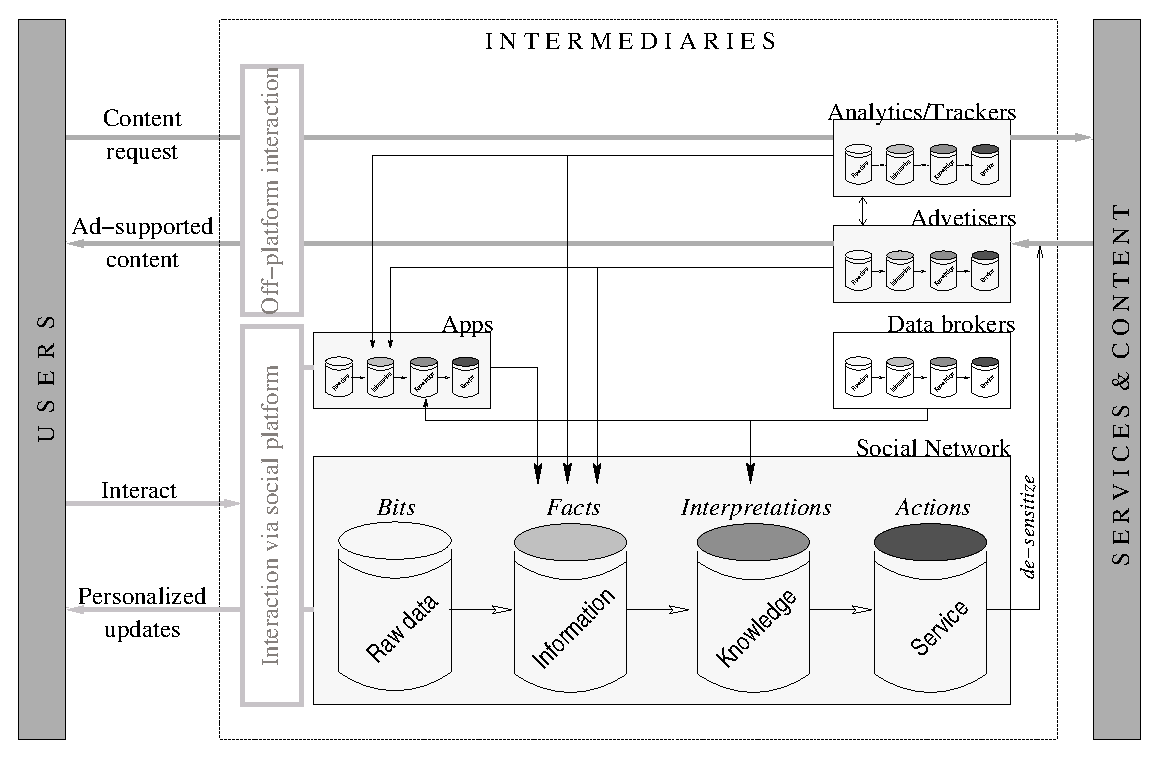
\epsfig{file = business-model.eps, width = 0.8\textwidth}}
  \caption{Business model of social networks
    ($record \rightarrow interpret \rightarrow monetize$).}
  \label{fig:business-model}
\end{figure*}

\subsection{The OSN platform}
\label{sec:osn-platform}
\noindent Facebook has evolved from a social network to an
intermediary with a bouquet of overarching services that supplement
its core business of collecting, interpreting, and monetizing user
data. So far, it has been successful in pushing its users to accept
evolving privacy norms by offering them compelling user experience
through convenience\footnote{The tyranny of convenience, Tim Wu, NYT,
  16/2/18.\\ https://www.facebook.com/zuck/posts/10104899855107881},
personalization. In this section we explore the stakeholders of this
platform and how they collaborate in its business model.

\paragraph{Users.}
Users are the largest part of the platform. They are represented as
nodes on a graph, called social graph, in which \textit{labelled}
edges represent relationships between nodes. Users'
\textit{interactions} within their reachable neighborhood and beyond,
with the nodes introduced by the NewsFeed, builds behavioral profiles
of users. NewsFeed is Facebook's intelligent algorithm that
prioritizes social updates from a user's neighborhood. If we assume
that each object (e.g., content like photos, also represented as a
node) on the social graph has a category type associated with it,
like: education, finance, food, sarcasm, celebrity, etc., then a
subject's interaction with these objects determine the probability of
interest the subject may have in such categories. Each interaction of
a subject with its neighborhood node improves the confidence level of
subject-category mapping. The objective of NewsFeed algorithm is to
increase subjects' interaction with variety of content categories
\cite{ipip-3200} so that a rich user profile can be built. Such a user
profile is pivotal in determining relevancy of updates to the user and
also to match the user with an advertiser advertising for a subset of
such categories \cite{fb-ad-categories}. Higher the engagement of the
user, higher the confidence value in categorizing the user.

\paragraph{Apps.}
The platform gives a general purpose connectivity and interaction
mechanism to the users, whereas the Apps give a context to user
profile. App serves a specific functionality (e.g., finance,
education, dating, et al.) to its users and that functionality is a
stronger measure of categorization. Apps can opt for monetization by
serving advertisements to the users via the App. Apps obtain analytics
over their users interactions (see
Figure~\ref{fig:business-model}). The analytics information contains
attributes (like mobile advertisement ID, Facebook UID, email, phone,
device info, location, etc.) that can uniquely measure interactions of
App users. To advertise itself, or to persuade its existing users the
App shares its analytics with advertisers to reach the existing and
new users.

\paragraph{Analytics and trackers (Pixel).}
Pixel is a micro-targeting framework
(\url{fb.com/business/learn/facebook-ads-pixel}) that uniquely
identifies users of the platform and also users
off-the-platform~\cite{social-plugins,web-never-forgets}. This is a
script that generates a unique tracking number each time a defined
event occurs. The events could be as simple as loading a website or a
user selecting a product in her cart. The unique number concatenated
with cookie at user side tracks the user event by event. These user
behavior analytics are availed by the platform to the advertisers so
that advertisers can measure the impact of their advertising
campaigns.

\paragraph{Advertisers.}
The platform's ability to find relevant audiences for a specific
category/issue brings advertisers to the
platform\footnote{https://developers.facebook.com/docs/marketing-api/reference/custom-audience}
. Advertisers build advertisement campaigns by requesting specific
audience type from the platform against a fee. To compose an audience
request, advertiser
uploads\footnote{https://www.facebook.com/business} data fields that
get compared against the user profiles built by the platform. Upon
evaluating the scope of the campaign being submitted by an advertiser,
the platform may refuse to execute the campaign; if i) it could not
find any users for the requested audience type, or ii) the requested
audience size is too small. However, the advertisers are allowed to
micro-target a specific audience that is already engaged with a
campaign. Advertisers do so by defining events inside the
Apps/services and triggering corresponding actions upon event
actuation. For example, list of users who have browsed a product
inside the App but did not checkout, visit a particular website.

\paragraph{Platform owner (FBAN).}
Facebook Audience Network (\url{fb.com/audiencenetwork}) is the core
component of the platform and has complete access to users' profiles
generated to date. It has its own data-set and models that are built
by tracking users (analytics) and their meta-data from other sister
platforms (like WhatsApp, Messenger, Instagram). It accepts audience
requests and based on corroboration of uploaded data by advertiser
with its proprietary data-sets, it generates a target audience. It
incorporates data from data-exchanges (like acxiom, datalogix, datamarket, datastreamx,
equifax, bluekai, epsilon) and data from government departments (like
land/property records, census, electoral roll) for its users, which
help enrich users' existing profiles.\\

\noindent Data platforms like Facebook whose business model is based
on advertisement have a similar schematic design that we saw
above. The platform provides a compelling service (like email, chat)
in return of a consent from its users to access their data and observe
their interactions. The platforms compete with each
other~\cite{data-goliath} to attract advertisers by innovating ways
for advertisers to track and target existing and new
customers. Innovations include features providing convenience,
personalization either by the platform or via the App ecosystem. The
core characteristic of these platforms is \textit{labelled data
  collection} where users voluntarily label themselves either through
the generic features of the platform or through the specific features
of the Apps they authorize. Users are given a set of options to
control the access to their data by other users, Apps, and to some
extent advertisers. In the following we shall see the access control
provided by Facebook platform.

\subsection{Access control}
The Facebook data platform appears to have a somewhat hybrid, ad-hoc
access control system in place. It is primarily designed for speed and
ease of feature integration. To do so, it organizes its users, their
content, and their relationships as a social graph~\cite{fb-tao} where
nodes represent subjects \& objects like users, Apps, content and
edges represent relationships among the nodes. Nodes have
types\footnote{developers.facebook.com/docs/graph-api/reference} and
can be queried by other nodes (of type user and App) directly or
indirectly. Graph
queries\footnote{developers.facebook.com/docs/graph-api/explorer}
return data only if the access policy specified at the node is
conformed by the querying node. Reachability is the primary condition
for access. There is a logical hierarchy among the node types on the
platform. It is designed in a way that higher a node in the hierarchy,
larger is the access to data. In other words, an App type of node can
make far richer types of queries on the social graph than a User type
of node -- an thus far can collect higher volumes of user
data. Figure~\ref{fig:access-hierarchy} depicts the volume of data on
the platform and the access hierarchies among the stakeholders of the
platform. Since the evolution of data begins with the users creating,
sharing, and interacting with the data, users are said to be the
primary owners of the data and therefore we list out the access
control methods available to them.
\begin{figure}[!tp]
  \centering
  {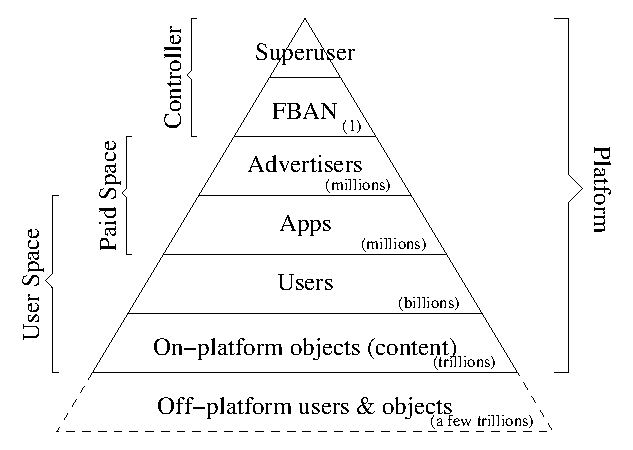
\epsfig{file = hierarchy.eps, width = 6.5cm}}
  \caption{Facebook platform: hierarchy of access.}
  \label{fig:access-hierarchy}
\end{figure}
\paragraph{User to user.} User nodes on the social graph can query
other user nodes and their objects (nodes depicted at the bottom of
the pyramid in Figure \ref{fig:access-hierarchy}) in accordance with
the policy specified at the target node. Facebook allows its users to
specify access policies over their objects using a mix of intensional
and extensional labels like ``Friends'', ``Family'', ``Friend of
friends'', et al. This type of natural labeling nomenclature allows
users to organize their social relationships as they do in offline
world. This communicates the affinity/strength of the edge between
nodes; thus, inversely a node's ability to influence the node at the
other end of the edge. Therefore the list of ``Friends'' of a user
becomes a valuable information and Facebook provides means to protect
such objects from unauthorized access. However, in~\cite{vtp-rks-fb1}
the authors show that the access policies on the Facebook platform do
leak user data despite correct policy specification by the users on
their objects.

%test\footnote{inteltechniques.com/osint/menu.facebook.html}
\paragraph{User to app.} The user nodes cannot query the App nodes
above in the hierarchy whereas the App nodes can query the User nodes
directly and their objects indirectly. An App's access to user nodes
is not controlled by the natural labels, as provided for user-to-user
access control, but through an explicit list of permissions (total 48
such permissions are available in v2.12 of Facebook's graph API) that
user confers on the App at the time of installation. The access
control for user data by Apps is designed for facilitating
functionalities of the Apps. Users give a set of permissions as
requested by an App to obtain the functionality. Whatever
transactional/observational data is generated, during the course of
App functionality usage, is not controlled by the user. Facebook
prompts users that by installing an App, a user abides to the privacy
policy of the App. There are 3 broad categories of Apps: i) Apps that
rely on FB for authentication (SSO), ii) Apps that modify the social
graph with consent from user, and iii) Apps that tailor user
experience based on the social graph of its users. The first two
categories, by design, shares the user activity with the platform;
whereas in the third category the user activity is recorded outside
the platform. User's permissions to Apps are perpetual and the data
availed by Apps are not governed by FB's privacy policy. Furthermore,
the permissions to Apps override the access controls expressed by
users in user-to-user layer. For example, a post by a user with policy
``Only Me'' is accessible by an
App. In~\cite{isrdc-tr-2017-rks-vtp-privacy-fb-apps} the authors list
out scenarios in which Apps either breach users' stated policies or
simply undermine user's sensitive information for which the platforms
does not provide any measure of protection. For example, an App can
find out what other Apps the user has installed.
%
%
\paragraph{User to advertiser.} Advertisers too are provided with UIDs
but these are not query-able as the UIDs of users and Apps. Neither
the advertising nodes can query the nodes in ``User Space'' as shown
in Figure~\ref{fig:access-hierarchy}. However,
advertisers\footnote{https://lifehacker.com/5994380/how-facebook-uses-your-data-to-target-ads-even-offline}
get indirect access to users' behavior data through the analytics
available to Apps and off-platform services (websites, and Apps). The
only control users get over
advertisers\footnote{https://www.facebook.com/ads/preferences},
regarding advertisers' access to user data, is by disassociating with
them.
%
%
\paragraph{User to platform.} By virtue of being the owner of the
platform, the superuser node can query any other node, on the social
graph, without any access
restrictions\footnote{motherboard.vice.com/en\_us/article/kzxdny/facebook-investigating-employee-stalking-women-online}.

Users implicitly trust the platform and therefore are comfortable with
being observed by the platform. Users may not invoke similar level of
trust with the Apps that are supported by the platform and therefore
the platform provides its users a choice to control the set of
permissions an App can obtain to access user data. \textit{The notion
  of privacy of a subject comes to fore only in the presence of an
  observer/violator who knows the subject.} And therefore, the
user-to-user access control is relatively expressive than the
user-to-App or user-to-advertiser access control.

In light of the recent Cambridge Analytica~\cite{fb-ca-lse}
revelations, this falsely perceived \textit{status quo} about privacy,
that existed for past decade, is being questioned widely. This is not
a one off scenario of users' privacy breach but it is due to lack of a
uniform platform-wide access control model. The access controls are
implemented layer-wise, where policies in one layer may contradict
with policies in another. As a response to Cambridge Analytica
incident, Facebook maintains that it will review and limit Apps'
access to user data and also highlights that users are owners of their
content and can control who can access these content. What it is
curiously missing is who can access the meta-data and behavioral data
about user interactions. This position is tenable, for now, because
there is an absence of Internet-wide agreement about \textit{who owns
  the meta-data -- data about data} and scope of data-usage, which is
a challenge to verify, though defined.

Facebook allows its users to delete their accounts. Through this paper
we would like to bring the reader's attention to the following
questions: i) How effective a user's decision is to delete her account
in order to avoid her being profiled? ii) Post deletion, is it
technically possible for the platform to uniquely identify the user?
iii) What are the technical limitations to enforce GDPR's ``right to
be forgotten'' intent?

Before we get into the analysis of these questions, it would be
appropriate to understand the characteristics of information, digital
transactions, the life-cycle of personal data, its mutation into
other types in presence of other auxiliary data, and the risks of
de-identification of de-sensitized/anonymized
data~\cite{paul-ohm-accretive}.

%\section{DATA LIFE-CYCLE, LINKABILITY}
%\section{DATA, METADATA, LINKABILITY}
\section{LIFE-CYCLE OF PII IN OSN}
\label{sec:life-cycle}
\noindent In this section we take the reader through a brief journey
of a user's data on OSN platform -- Facebook.

PII~\cite{nist-pii} is ``any information about an individual
maintained by an agency, including i) any information that can be used
to distinguish or trace an individual's identity, such as name, social
security number, date and place of birth, mother's maiden name, or
biometric records; and ii) any other information that is linked or
linkable to an individual, such as medical, educational, financial,
and employment information.'' To distinguish an individual is to
identify an individual.

Identifiers distinguish a user (or a group of users, or a passive
object) from another. Each unique entity that needs to be interacted
with has an identifier, e.g., name. Identifiers may have attributes
like postal address, city name, date of birth. Attributes are a
generic class of identifiers, which do not identify a subject on its
own but in presence of its association with a subject improves the
uniqueness of subject identification. Observer is an entity that has
knowledge of identifiers of subjects and it may assign private
attributes to subjects based on their activities under
observation. For example, an ISP may legitimately assign attributes
like gamers, bankers, student, etc. based on the online activities of
its customers. Observer may develop data models based on its
customers' online behavior and may devise a method to predict
attribute/category for an unknown subject when that subject's log of
online activities is fed to the model. Therefore, the potency of an
observer is proportional to the volume of data it has access to. When
an attribute is unique to a subject then the attribute is equivalent
to PII in the given context. For example, if there is only one person
with a specific DoB in a database (knowledgebase) then that attribute
uniquely identifies the subject it is assigned to. If there are more
than two subjects that have same DoB, then the probability of
correctly associating a subject to an action reduces to half, and
likewise. Whereas instead of one attribute, two attributes of subjects
are considered under the same observation model, the probability of
subject identification greatly increases. Users neither have knowledge
about potency of their observers nor sufficient motivation to
judiciously reveal their attributes while online. \textit{Level of
  privacy is a loose measure of asymmetry of motivation, ability
  between an observer and the subjects being observed.} An observer
(advertiser or its collaborator) is financially motivated to identify
its audience and has technical ability (via the platform) to do so;
whereas, the users are motivated to get functional benefits of the
free service being provided, until and unless adversely affected.
\begin{figure}[!htp]
  \centering
  {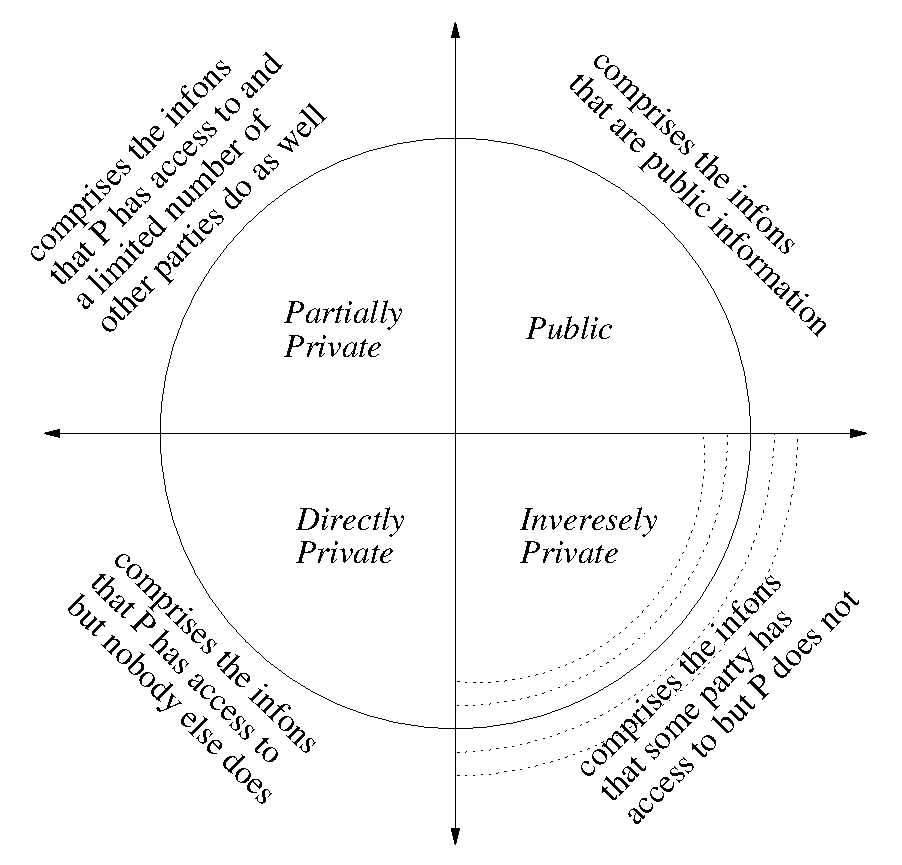
\epsfig{file = personal-info-classification2.eps, width = 0.4\textwidth}}
  \caption{Classification of PII (infon) of subject P.}
  \label{fig:personal-info-classification}
\end{figure}
\paragraph{Coarse classification of PII.}
In~\cite{inverse-privacy}, the authors classify personal data (infons)
of a subject into 4 flat categories as shown in
Figure~\ref{fig:personal-info-classification}. Examples of these types
of infons are: \textit{Public} -- name, email, phone; \textit{Directly
  Private} -- passwords; \textit{Partially Private} -- salary, blood
group; \textit{Inversely Private} -- mobile location logs. We term
this classification coarse because in absence of context the above
examples may fall in multiple classes. For example, passwords can be
categorized as partially private either, because the validator retains
a copy of the password. Likewise, an individual's credit rating can be
categorized as inversely private until that individual obtains a copy
upon payment. Therefore, context is an important aspect in accurate
categorization of PII -- this is what Facebook's social graph does --
it records all the previous interactions of a subject and changes the
state of the social graph so that new state is available to all other
nodes of the graph.

In the following, we walk through the process of how users' PII on an
OSN platform gets transformed from governable verbatim strings to
ungovernable diffused data. The process is abstracted out in 4-steps
and depicted in Figure~\ref{fig:data-life-cycle}.
%
\begin{figure}[!h]
  \centering
  {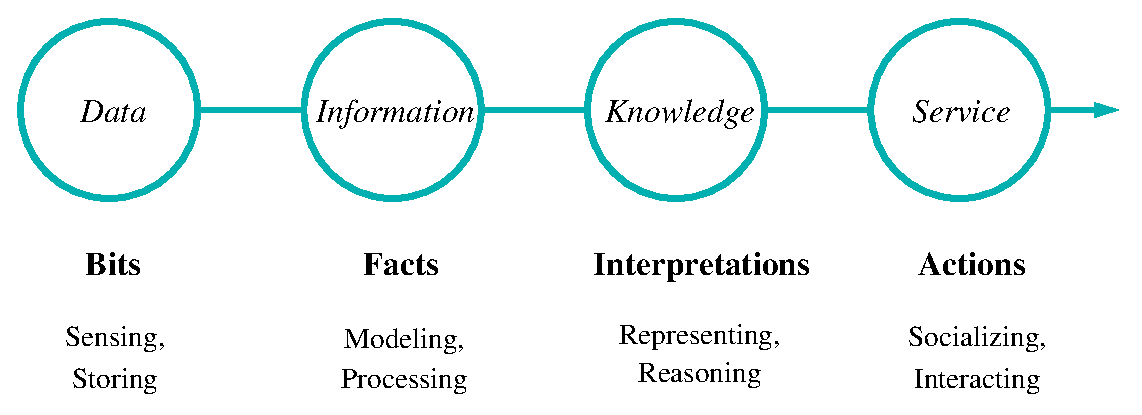
\epsfig{file = data-life-cycle.eps, width = 7cm}}
  \caption{Abstractions along the information value chain.}
  \label{fig:data-life-cycle}
\end{figure}
%
\paragraph{Voluntary labeling (sensing, storing of data).} When a user
signs-up with the platform by providing her personal details, the
platform assigns a 64-bit unique ID (FBID) to the user and is
represented as a node on the social graph. FBID acts as a primary
identifier on the platform and user fills out various personal details
(DoB, affiliation, city, languages) as attributes to the FBID
node. User node's edges to other nodes represent relationship of a
specific type: social affinity (friends, family, acquaintance, groups,
et al), object ownership (photos, post, video, et al), actions
(check-in, like, comment, tag, events, et al), and installation of an
App. All these possible edge formations by a node is used for labeling
the node according to the type of the peer node. For example, user
installing a sports App will label the user in ``sports''
category. The user ``like'' a post of category ``sport'' by other user
will reinforce the labeling. Thus, a node's category influences the
categories of the nodes interacting with it. The platform labels the
object nodes (content, location, Apps, groups) to determine interests
of its subjects when they voluntarily interact. Apps may have their
own private labels, which they may or may not share with the platform.


\paragraph{Observational labeling (modeling, processing of information).}
The platform observes and records its users activities on-platform and
off-platform (through Pixel, for example). These observations include
facts like IP address, type of mobile OS, type of
browser~\cite{fb-browser-extension-detection}, active time on
platform, active time on other
platforms\footnote{https://www.wsj.com/articles/facebooks-onavo-gives-social-media-firm-inside-peek-at-rivals-users-1502622003},
call logs, browser logs, location history,
etc~\cite{big-brother-watching}. All this factual information along
with the voluntary labels/categories form rich profiles about users
and also group of users. Further enrichment and fortification of
information is done by correlating data from external
sources\footnote{https://www.facebook.com/help/494750870625830} like
credit-rating agencies, census data, electoral rolls. Both the Apps
and platform track user behavior by modeling events in the
interactions of users on/off the platform. This analytics is processed
and compiled as formatted information such that it can readily be used
to re-target the users towards attending incomplete events; for
example, a user added items to shopping basket but did not check-out,
so re-targeting such users to complete payment event is an objective. A
user who has history of adding items to basket but not checking-out is
not the audience advertisers are interested in.

%\paragraph{Inferred labeling.} device id, browser id
%\paragraph{Correlation via external data.}

\paragraph{Mutation \& diffusion of data (representing, reasoning of
  knowledge).} Advertisers are interested in getting a high conversion
rate for their advertising budget. Personality of a user is a strong
measure to anticipate her behavior. The user profiles containing rich
sets of labels are then
synthesized~\cite{kosinski-youyou,kosinski-likes} into valuable
individual personality
traits\footnote{https://ipip.ori.org/AlphabeticalItemList.htm} --
which in its abstract form is represented by OCEAN~\cite{ocean-costa}
or Big Five\footnote{http://www.outofservice.com/bigfive/} score. Thus
the verbatim user profile tuples $<$FBID, labels$>$ get mutated into
$<$FBID, labels, OCEAN$>$. Then the users can be dB-identified and
organized according to their personality traits so that advertisers
can rent it out to construct their tailored audience for a specific
campaign. Each campaign has a context and FB-AN does the placement of
advertisement since it has complete knowledge -- user profiles,
traits, and the context. Expertise from other well-known psychometric
models is used to further synthesize the knowledgebase of FBAN to build
new reasonings~\cite{parsinomious} about users' behavior prediction in
presence of certain events that are triggered either on the platform
or elsewhere.  This is how verbatim a user's PII data gets mutated and
be diffused in information value chain, as knowledge, as shown in
Figure~\ref{fig:data-life-cycle}. It is possible that same
knowledgebase can be constructed using two different datasets. In
other words, exclusion or inclusion of a small quantity of input data
does not change the knowledgebase substantially.

Users are made available the logs of their actions on the platform but
not within the Apps. The inferred categories\footnote{In 2016,
  ProPublica collected more than 52,000 unique attributes that
  Facebook has used to classify users~\cite{fb-ad-categories}} that
are labelled against users' respective FBIDs are neither made
available to users.

\paragraph{Monetization of data (actions: putting knowledge into use).}
Facebook's overarching \textit{sensing, recording} platform
(Section~\ref{sec:osn-platform}) continuously does 3 tasks in tandem
to consolidate its hold on users' information value chain: i) collect
\& classify user PII data/actions, ii) correlate data/actions with
other facts to build/improve profiles, and iii) dynamically build
audiences as per contexts specified by its customers. In the process
the users PII data and actions are continuously transforming across
the information value chain and getting diffused into actionable
knowledge. The omnipresent, overarching ecosystem of Facebook, through
its platform components and analytical feedback loop from
internet-wide content collaborators, is a real-time context delivery
service. FBAN's knowledgebase along with platform's real-time context
prediction capability helps Facebook to attract advertisers,
governments, and persuaders to build/identify tailored
audiences. However, Facebook takes precaution to prevent its customers
from tailoring audience that has size smaller than 100. The same
knowledgebase is also used in Facebook's NewsFeed algorithm, which is
famous for its prioritization of relevant updates to a user.

This brings us to the most interesting question in PII's life-cycle:
is it possible to identify a user with the help of a
knowledgebase/model that is trained on the data involving the user's
PII? In the following section, we shall argue about it in affirmation
while explaining the efficacy of soon to be enacted GDPR for EU
subjects.



% \subsubsection{User profiling/labeling}
% \paragraph{Profiles.} All individual user profiles are further
% enriched and attributed by the insights obtained from platform
% analytics and plausibly external public/private
% data-sets\footnote{www.facebook.com/full\_data\_use\_policy}
% (For Indian users, Facebook tried to link their Aadhaar numbers with
% their profiles. Aadhaar numbers are not secret but are used in various
% financial and public services delivery).

% \subsubsection{Event association}
% \subsubsection{Personalization}
% \subsubsection{Audience measurement}
% \subsubsection{Profile enrichment/enforcement}
% \subsubsection{Psychometric profiling}
% \subsubsection{Behavior prediction, econometrics}


% \section{GDPR \& DATA GOVERNANCE}
\section{EFFICACY OF GDPR IN OSN}
\label{sec:efficacy}
\noindent GDPR's tenets will certainly change how users PII is
collected, processed, and disposed off. Users will have to be
explicitly consented, informed, and allowed to access/delete their
PII. Any entity that legally interacts with subjects across EU are
covered by GDPR with certain
exceptions\footnote{https://gdpr-info.eu/recitals/no-52/}, which does
not cover OSNs.  Handlers of PII are categorized as: i) \textit{data
  processors} -- entities processing data on behalf of the controller,
and ii) \textit{data controllers} -- entities deciding what personal
data must be processed and how processing will occur. Facebook acts as
both\footnote{https://www.facebook.com/business/gdpr} the controller
(for its users) and the processor (for its millions of Apps; where
Apps act as the controller of user data) of PII. Facebook Apps in
their data controller role need to get explicit consent from their
users to collect and use the user data, which might
directly/indirectly be available to underlying platform of Facebook
and thus gets mutated and diffused into FBAN's knowledgebase. Keeping
this in mind, the efficacy of \textit{right to be
  forgotten}\footnote{https://gdpr-info.eu/art-17-gdpr/} is analyzed
below.

\paragraph{Right to be forgotten.} When a user invokes this right, the
data controller and processor have to delete all the data they have
collected (not only the PII) that can directly or indirectly uniquely
identify the user. In case of Facebook, the \textit{spirit} of this
GDPR article is that the user should not be remembered for any of the
services offered by Facebook. In \textit{letter}, Facebook will delete
all the directly/indirectly identifiable data about the user from its
information value chain. But as described in previous section, the
identifiers (FBID, attributes, labels) that are associated with a user
exist in verbatim form only till the modeling/processing stage of
platform's information value chain. Beyond that stage it exists in a
diffused form, as knowledge, which would have been the same even if
the user had not joined the platform. Figure~\ref{fig:data-governance}
shows the effective boundary of GDPR's delete operation on an OSN
platform like Facebook. In other words, right to erasure will delete
only the PII, voluntary labels, observational labels but it cannot
force the platform/Apps to reverse the knowledge created using
machine-learning models trained using user's data.
%
\begin{figure}[!h]
  \centering
  {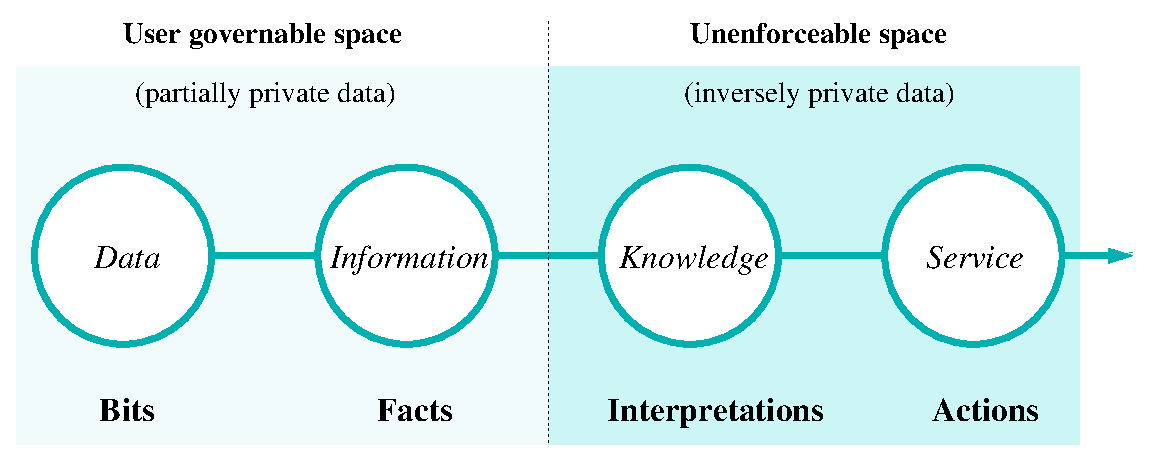
\epsfig{file = data-governance.eps, width = 7cm}}
  \caption{Information value chain: scope of regulation}
  \label{fig:data-governance}
\end{figure}

Post invocation of right to erasure by an user, the user continues to
get identified by her metadata (IP, locale, time-zone, behavioral
fingerprints, hardware fingerprints, et al) and platform's capability
to
track\footnote{\href{https://www.theregister.co.uk/2018/04/17/facebook_admits_to_tracking_non_users/}{theregister.co.uk/2018/04/17/facebook\_admits\_to\_tracking\_non\_users/}}
non-users~\cite{social-plugins,web-never-forgets} across the affiliate
services/websites that are associated with the platform. This tracking
data allows Facebook to determine context of the non-user, which is
sufficient to match the non-user's attention to an advertiser with as
much relevance as when the user was associated with the platform. And
it will be technically not feasible to prove that Facebook has used
PII to match the user with an advertiser. In fact, the user will be
better off by staying associated with the platform instead of being
forgotten by the platform because while associated with the platform
the user can at least control her ad preferences.

Even if Facebook wants to honor user's right to be forgotten in
\textit{spirit}, it will have to track such users in order to instruct
FBAN to do so. This could be easily achieved by issuing such users a
``do not track'' cookie. But this will break the business model of
Facebook as losing the context of user's attention will reduce the
click-through rate for advertisements. In other words, \textit{right
  to be forgotten} is the least effective tenet of GDPR. We are all
witness to the rampant disregard for ``Do Not Track'' setting in
modern browsers. What this tenet of GDPR may achieve with limited
success is: suspension of perpetual compilation of user's personality
and behavioral traits.

% regulation will benefit the incumbent: people trust known brands

% in order to curb fake accounts on the platform, users will be asked to
% link themselves using a legal identity. The efforts to regulate data
% platforms are indirectly strengthening the platforms.

\section{DISCUSSION}
\label{sec:discussion}
\noindent There is a technological imbalance among the stakeholders of
our digital economy. The platforms have attained technical superiority
in data collection, processing and actively influence the design of
fundamental interfaces to Internet (browser, DNS, mobile OS, Apps) to
further consolidate\footnote{Net neutrality blocked ISPs from
  providing services subsidized with advertising.} their data-driven
business model: \textit{record everything} $\rightarrow$
\textit{interpret} $\rightarrow$ \textit{monetize and persuade.}

Advertisers' primary motivation/aim is to reach their intended
audience with minimum expenditure. The expenditure is optimum when
there is an exact match, in other words, precision targeting is
inevitable. OSNs have created the ability to identify their users for
specific criterions that advertisers are interested in. Through OSNs,
the \textit{motivation} of advertising industry is easily achieved due
to the technical \textit{ability} of OSNs to accurately find the
users. On the other hand, users typically lack the motivation and
ability to make elaborate privacy decisions. Furthermore, for the
platform/advertiser, the cost of making a wrong probabilistic guess
about intended target is negligible whereas, for the target/user, it
is costly to get identified.

GDPR has stiff financial penalties for laxity in personal data
handling. However, provenance is difficult given the fact that a data
controller (an App) on Facebook platform, by design interacts with the
underlying social graph. Depending on the design of the App, partial
or full data of App user is recorded on Facebook's social graph. The
data then propagates further in platform's information value chain. It
is easy to create an App and start collecting user data without much
of practical liabilities. This is because any user can create an App.
Facebook has introduced a concept of Scope\_ID that issues local
identifier to App users such that the identifier can only be valid
within the scope of the App. Users cannot be tracked for their
activities across the Apps. However, FBAN can resolve the Scope\_IDs
of all Apps. It will be interesting to see what changes Facebook will
usher in to its platform to be compliant with GDPR while acting as a
data processor for its Apps. We contend that the relationship is not
so distinguishing between Apps and Facebook platform as controller and
processor. 



%appropriate to deal with today's technological landscape

% \paragraph{Data provenance is costly.} Therefore accountability is hard to enforce.
% %\subsection{IoT, ambient computing}
% \paragraph{Usage control.}
% %\subsection{Information flow control}
% %\subsubsection{Labeling of data to define context}
% \paragraph{RWFM for IFC enforcement.} \cite{rwfm}
% \paragraph{Communicating consent through 5-star rating.}
% Easier privacy policies that help users understand what they are
% agreeing to. Analogy: 5-star rating of electrical appliances help
% users understand power consumption of the device; similar effort to
% communicate privacy policy to users is important.


In presence of ubiquitous tools like big-data analytics and deep
neural networks, preserving privacy appears to be a herculean
task~\cite{unique-mall,unique-crowd}. To address this challenge
coherently, we need to undertake a SoK for identifiers. Because it is
their usage beyond the perceived scope of their utility that leads to
potential privacy breaches. The SoK should put forward a framework for
the use of identifiers in terms of their scope, contextual
availability, temporal validity, linkability -- and the effects of
these parameters on each other. Architects of online services have
service functionality and user convenience as primary design
criteria. Providing them a methodology to judiciously use the above
mentioned parameters with an understanding of their costs and benefits
to the system they design.


\section{CONCLUSIONS}
\label{sec:conclusion}
\noindent To pursue is an innate desire and manifests in many
ways. Advertisement is one of such external manifestations of
persuasion. OSNs with their close proximity to user's day-to-day
activities have become a real-time gauge of user's mindset --
necessary for effective and quick persuasion. A business model has
evolved in which users trade their private data for convenience and
ad-supported services. The trade-offs continue to favor the platform
owners and their techniques to track user activities have brought in a
privacy anxiety and helplessness to users -- primary stakeholders of
online ecosystem. A lack of transparency in collection, processing, and
usage of of personally identifiable data by OSNs is undermining trust
in online services. As the facade of self-regulation has failed
spectacularly, GDPR is the first right step to address this
crisis. However, an important tenet of this regulation, \textit{right
  to be forgotten}, has very little efficacy in OSNs with their
prevalent omnipresent \textit{data sensing} platform. We have argued
that to implement this tenet in its \textit{spirit}, platform's
business model breaks and we have little evidence that self-regulation
has worked. To bring in accountability, transparency, and competitive
innovation; OSNs should either treat the Apps as their own extensions
or relinquish its role of data processor when a data controller brings
in data of users (to the platform for processing) who have invoked
their right to be forgotten on the platform. But, will it be naive to
expect voluntary declaration of \textit{conflict-of-interest} from the
class of entities who have failed to self-regulate for decades?


% Their
% business model of collecting minutest details of user activity online
% to monetize it using sophisticated, intrusive models for user behavior
% prediction has reached an unsustainable level. It is threatening the
% very ecosystem on which it has thrived.

% User tracking and context-based user persuation are not only
% profitable activities but are also 

% There are hardly any websites/online services that do not do
% some sort of analytics and 

% Having such a framework, privacy-by-design models can strive for
% transparent, accountable, PII data-governance.

% ethics, law, technology. metaphysical realm.

\nocite{pbd-7,eu-gdpr,Dixon2017,privacy-paradox,business-of-personal-data,contextual-integrity,vtp-rks-fb2}

\nocite{kosinski-facebook-personality,linkability1,sso1,sso2,inverse-privacy,ftc-2012,what-matters-to-users}

%\vfill
%\newpage
\bibliographystyle{apalike}
{\small
\bibliography{gdpr}}


% \section*{\uppercase{Acknowledgements}}

% \noindent If any, should be placed before the references section
% without numbering. To do so please use the following command:
% \textit{$\backslash$section*\{ACKNOWLEDGEMENTS\}}


% \begin{figure}[!h]
%   %\vspace{-0.2cm}
%   \centering
%    {\epsfig{file = SCITEPRESS.eps, width = 5.5cm}}
%   \caption{This caption has one line so it is centered.}
%   \label{fig:example1}
%  \end{figure}

% \begin{figure}[!h]
%   \vspace{-0.2cm}
%   \centering
%    {\epsfig{file = SCITEPRESS.eps, width = 5.5cm}}
%   \caption{This caption has more than one line so it has to be justified.}
%   \label{fig:example2}
%   \vspace{-0.1cm}
% \end{figure}

% \section*{\uppercase{Appendix}}

% \noindent If any, the appendix should appear directly after the
% references without numbering, and not on a new page. To do so please use the following command:
% \textit{$\backslash$section*\{APPENDIX\}}

\vfill
\end{document}

\begin{comment}
  have attained pervasiveness and thus be very difficult to regulate
  or remove.

  Digital forms of identity systems, when fully developed and
  deployed, are expected to be more powerful and efficient tools of
  identification than legacy paper systems. The power and efficiency
  proffered by such tools, both pose and mount a great urgency to
  identify, and to mitigate modern risks associated with system breach
  and the compromise of vital information in those identity systems,
  and to ensure that digital identity systems do not become tools of
  suppression, oppression, exclusion, or discrimination.
  [Dixon 2017]

  Your privacy is only as good as your friend's privacy.

  The study's findings indicating the power of placement and navigation ease
  are consistent with consumer behaviors tech firms already know
  well.

  intermediaries -- Facebook/Google (platforms)

  consumer behavior, incentives, navigation/placement, convenience,

  extrapolate,

  convenience / seamless experience = user identification / SSO -- all
  of them want to be authentication platform.

  risk of re-identification of anonymous personal data

  contextual and personalized advertising

  Facebook Tracks and Traces Everyone: Like This!

  It has become cheaper to collect and process data.

  PII's malleability [The PII Problem: Privacy and a New Concept of
  Personally Identifiable Information]

  

  Efforts to repackage pervasive surveillance as innovation -- under
  the moniker ``Big Data'' -- are better understood as efforts to
  enshrine the methods and values of the modulated society at the
  heart of our system of knowledge production. In short, privacy
  incursions harm individuals, but not only individuals. Privacy
  incursions in the name of progress, innovation, and ordered liberty
  jeopardize the continuing vitality of the political and intellectual
  culture that we say we value. [What Privacy Is For, Harvard Law
  Review, Vol. 126, 2013]

  role of identifiers -- A rose by any other name would smell as sweet
  [William Shakespeare]

  myriad of services collect, analyze, use, and exchange users'
  personal information

  we live in a world dominated by inverse privacy is not the invasion
  of privacy but the gross disparity in the capability to take and
  keep records.

  emotional intelligence

  align audiences

  flight records for Jeff Bezos's private jet are hinting at Amazon's HQ2 choice

  Hedge Funds Strike Paydirt on Actelion Deal After Tracking J\&J's Jet

  https://emotionresearchlab.com/

  https://newsroom.fb.com/news/2018/04/new-privacy-protections/

  https://newsroom.fb.com/news/2018/04/data-and-advertising/

  Advertisers need:
  - guessing purchase intent
  - 

  \footnote{\href{https://newsroom.fb.com/news/2017/11/our-advertising-principles/}{newsroom.fb.com/news/2017/11/our-advertising-principles/}}

  The tech giants came to prominence with better products and services
  that unseated their heavily-regulated rivals, those in state-owned
  television, pay television, radio and print. Yet once the web firms
  gained critical mass, they blocked potential competitors through
  classic telecom rules like ``network neutrality'' obligations and
  anti-discrimination policies that were applied to the telecom
  operators but not to
  them. [https://debates.economist.com/debate/should-regulators-break-tech-giants?state=opening]

  These rules have given the tech titans a free ride along the
  information highway. They force consumers to pay the full cost of
  their communications, rather than have it subsidized with
  advertising. Just as ads let Google and Facebook offer free
  services, it could lower the price of internet service. This
  innovation would give advertisers credible alternatives to the
  reigning platforms. That's why the tech giants and their
  globally-coordinated advocates have fought vehemently against it,
  aborting its birth by lambasting it ``non-neutral''.

  https://gdpr-info.eu/


  [Privacy Regulation and Market Structure]

  The techniques that Cambridge Analytica uses to produce its
  psychometric profiles are the cutting edge of data-driven
  methodologies first devised 100 years ago. The science of
  personality research was born in 1917. That year, in the midst of
  America's fevered entry into war, Robert Sessions Woodworth of
  Columbia University created the Personal Data Sheet, a questionnaire
  that promised to assess the personalities of Army recruits. The war
  ended before Woodworth's psychological instrument was ready for
  deployment, but the Army had envisioned its use according to the
  precedent set by the intelligence tests it had been administering to
  new recruits under the direction of Robert Yerkes, a professor of
  psychology at Harvard at the time. The data these tests could
  produce would help decide who should go to the fronts, who was fit
  to lead and who should stay well behind the
  lines. [https://www.nytimes.com/2018/03/22/opinion/democracy-survive-data.html]


  Data from Onavo's app has been crucial to helping Facebook track
  rivals and scope out new product categories
  [https://www.wsj.com/articles/facebooks-onavo-gives-social-media-firm-inside-peek-at-rivals-users-1502622003]

  https://www.nytimes.com/2018/03/22/opinion/democracy-survive-data.html

  https://ca-political.com/ca-advantage

  Credit bureaus have long been gathering information about our
  earnings, spending habits and loan-repayment histories to determine
  our credit-worthiness. Tech companies have taken this one step
  further, collecting data on our web-surfing habits and which numbers
  we call.  Via social media, we have volunteered information on our
  friends and our likes and dislikes, and shared family
  photographs. Our smartphones can know everywhere we go and can keep
  track of our
  health. [https://www.washingtonpost.com/news/innovations/wp/2017/09/29/why-we-need-new-regulations-to-protect-us-from-companies-like-equifax/?noredirect=on&utm_term=.64279bbfa794]

  privacy should be protected via property rights rather than via liability rules [Lawrence Lessig]

  Daniel J. Solove argues agains privacy as property right - innocuous
  actions leading to catastrophic outcomes. It is the totality of
  information about a person and how it is used that poses the
  greatest threat to privacy.

  Lookalike -- make multiple campaigns with one unique attribute
  category each time.

  PRIVACY: The Search is On!

  https://www.digitaltrends.com/web/ways-to-decentralize-the-web/

  Differential privacy guarantees that the participation of a single
  individual does not significantly change the result of a
  differentially private query. DP gives a measurable privacy
  guarantee which is future
  proof.
  [file:///Users/panini/Downloads/Jussi_Lepp%C3%A4l%C3%A4_Navigating%20Between%20Mathematics%20and%20the%20GDPR%3B%250BAnonymization,%20Pseudonymization,%20and%20Personal%20Data_August%2027,%202017%20at%201_04%20pm.pdf]

  GDPR does tighten existing consent requirements for processing personal data

  along with requiring data controllers are able to demonstrate that a
  service user whose personal data is being processed has given
  consent for that to happen.

  
\end{comment}